\documentclass[11pt]{article}

\usepackage[margin=1in]{geometry}
\usepackage{amsmath,amssymb}
\usepackage{booktabs}
\usepackage{graphicx}
\usepackage{microtype}
\usepackage{xcolor}
\usepackage{tikz}
\usetikzlibrary{arrows.meta,positioning}
\usepackage[numbers]{natbib}
\usepackage[colorlinks=true,linkcolor=blue,citecolor=blue,urlcolor=blue]{hyperref}

% ---------------------------------------------------------------------------
% Result macros — every number in the tables is defined here, sourced from
% results_squad/eval_results.csv and results/eval_results.csv in the artifact
% repository. Regenerate with `rag eval` (see Section 6).
% ---------------------------------------------------------------------------
% SQuAD-200 experiment (results_squad/eval_results.csv, warmed-up timing)
\newcommand{\sqAdRec}{0.935}\newcommand{\sqAdFone}{0.476}\newcommand{\sqAdEM}{0.440}
\newcommand{\sqAdLat}{0.447}\newcommand{\sqAdDocs}{4.93}\newcommand{\sqAdRr}{5.0}
\newcommand{\sqSiRec}{0.755}\newcommand{\sqSiFone}{0.641}\newcommand{\sqSiEM}{0.600}
\newcommand{\sqSiLat}{0.310}\newcommand{\sqSiDocs}{2.00}\newcommand{\sqSiRr}{0.0}
\newcommand{\sqCoRec}{0.995}\newcommand{\sqCoFone}{0.429}\newcommand{\sqCoEM}{0.410}
\newcommand{\sqCoLat}{1.270}\newcommand{\sqCoDocs}{10.00}\newcommand{\sqCoRr}{100.0}
\newcommand{\sqSimple}{21}\newcommand{\sqMedium}{169}\newcommand{\sqComplex}{10}
% Enterprise experiment (results/eval_results.csv, warmed-up timing)
\newcommand{\enAdRec}{1.000}\newcommand{\enAdFone}{0.917}\newcommand{\enAdEM}{0.773}
\newcommand{\enAdLat}{0.466}\newcommand{\enAdDocs}{4.91}\newcommand{\enAdRr}{9.1}
\newcommand{\enSiRec}{1.000}\newcommand{\enSiFone}{0.917}\newcommand{\enSiEM}{0.773}
\newcommand{\enSiLat}{0.266}\newcommand{\enSiDocs}{2.00}\newcommand{\enSiRr}{0.0}
\newcommand{\enCoRec}{1.000}\newcommand{\enCoFone}{0.917}\newcommand{\enCoEM}{0.773}
\newcommand{\enCoLat}{0.752}\newcommand{\enCoDocs}{10.00}\newcommand{\enCoRr}{100.0}

\title{\textbf{Hierarchical Fuzzy Query-Complexity Routing for\\Cost-Efficient Retrieval-Augmented Generation}}
\author{Arav Gulati\\\texttt{arav.gulati.ai@gmail.com}}
\date{}

\begin{document}
\maketitle

\begin{abstract}
Retrieval-augmented generation (RAG) systems conventionally apply a single,
fixed retrieval configuration to every query: the same retriever, the same
retrieval depth, and the same (optional) re-ranking stage, regardless of
whether the query is a two-word factual lookup or a multi-entity comparative
question. This forces a global trade-off between cost and quality. We present
an adaptive RAG architecture that estimates each query's complexity
\emph{before retrieval} using a two-stage hierarchical fuzzy inference engine
over six lightweight linguistic, knowledge, and reasoning features, and routes
the query to one of three retrieval policies (top-2 dense; top-5 hybrid
BM25+dense; top-10 hybrid with cross-encoder re-ranking). Unlike
classifier-based adaptive RAG, the router requires no training data, runs in
tens of milliseconds on CPU, and produces a fully interpretable rule-based
trace for every decision. The hierarchical design decomposes inference into
three 9-rule Mamdani subsystems plus a compact second-stage rule base that is
complete and monotonic by construction, avoiding the combinatorial rule
explosion of flat fuzzy systems. On a 200-question open-domain benchmark
derived from SQuAD, adaptive routing closes most of the recall gap between the
cheap and expensive fixed baselines while re-ranking only a small fraction of
queries; on a 22-question enterprise-policy benchmark it matches the expensive
baseline's answer quality (F1 $\enAdFone$, EM $\enAdEM$) at $1.6\times$ lower
latency, roughly half the retrieval volume, and $9\%$ cross-encoder usage. The
complete system runs offline on commodity CPU hardware with open models, and
all code, corpora, and evaluation artifacts are released for reproduction.
\end{abstract}

\section{Introduction}

Retrieval-augmented generation grounds a language model's answers in documents
fetched at inference time \citep{lewis2020rag}. Production RAG deployments
must choose a retrieval configuration: which retriever(s) to run, how many
passages to fetch, and whether to apply an expensive cross-encoder re-ranking
stage \citep{nogueira2019rerank}. Conventionally this choice is made
\emph{once}, globally. A cheap configuration (shallow dense retrieval)
minimizes latency and compute but misses relevant passages for hard queries; an
expensive configuration (deep hybrid retrieval with re-ranking) maximizes
recall but wastes most of its compute on queries that never needed it. Real
query workloads are heterogeneous: ``Who is the CEO?'' and ``Compare the
data-retention obligations under GDPR and CCPA for cloud providers processing
biometric data'' should not cost the same to answer.

Recent work adapts retrieval effort to the query, but typically by training a
neural complexity classifier \citep{jeong2024adaptive}, by fine-tuning the
generator itself to emit retrieval-control tokens \citep{asai2024selfrag}, or
by triggering retrieval from generation-time uncertainty
\citep{jiang2023flare}. These approaches require labeled training data,
model fine-tuning, or tight coupling to a particular generator.

We investigate a complementary point in the design space: a \emph{zero-shot,
fully interpretable} query-complexity router built from fuzzy inference
\citep{zadeh1965fuzzy,mamdani1975experiment}. Our system extracts six
lightweight features from the query alone---no retrieval, no LLM call---and
passes them through a two-stage hierarchical Mamdani engine whose output, a
continuous complexity score in $[0,1]$, selects one of three retrieval
policies. The fuzzy formulation contributes three properties that trained
routers lack: (i) it needs no training data or labels; (ii) every routing
decision is explainable as a small set of human-readable rules over named
linguistic quantities; and (iii) domain adaptation is a configuration edit (a
keyword list, a threshold) rather than a retraining run.

\paragraph{Contributions.}
\begin{enumerate}
  \item An adaptive RAG architecture whose retrieval policy is selected
        per-query by a hierarchical fuzzy engine over six pre-retrieval
        features spanning linguistic form, knowledge density, and reasoning
        type (\S\ref{sec:method}).
  \item A hierarchical rule-base design---three 9-rule expert subsystems plus
        a second-stage aggregator---that is \emph{complete} (every input
        activates at least one rule) and \emph{monotonic} (raising any
        subsystem's complexity never lowers overall complexity) by
        construction, verified by property-based tests
        (\S\ref{sec:hierarchical}).
  \item Two training-free, corpus-adaptive feature components that remove the
        approach's main hand-authored priors: a domain vocabulary derived from
        the corpus by contrastive TF-IDF (\S\ref{sec:domain}) and a
        syntax-aware, soft-scored intent detector (\S\ref{sec:intent}).
  \item An end-to-end open implementation on commodity CPU hardware (spaCy,
        scikit-fuzzy, MiniLM bi-/cross-encoders, BM25, Flan-T5), with an
        evaluation harness that reports quality \emph{and} cost jointly
        (\S\ref{sec:setup}).
  \item An empirical study on two corpora showing that fuzzy routing recovers
        most of the recall lost by cheap fixed retrieval at a small fraction
        of the cost of expensive fixed retrieval (\S\ref{sec:results}).
\end{enumerate}

\section{Related Work}

\paragraph{Retrieval-augmented generation.}
RAG couples a parametric generator with non-parametric memory
\citep{lewis2020rag}, typically via dense passage retrieval
\citep{karpukhin2020dpr} with bi-encoder embeddings \citep{reimers2019sbert},
sparse lexical retrieval such as BM25 \citep{robertson2009bm25}, or hybrids.
Cross-encoder re-ranking substantially improves precision at significant
compute cost \citep{nogueira2019rerank}; rank-level fusion methods such as
reciprocal rank fusion combine heterogeneous rankers robustly without score
calibration \citep{cormack2009rrf}.

\paragraph{Adaptive retrieval.}
\citet{mallen2023popqa} show that retrieval helps selectively and propose
popularity-based gating. Adaptive-RAG \citep{jeong2024adaptive} trains a
T5-based classifier to route queries among no-retrieval, single-step, and
multi-step strategies. Self-RAG \citep{asai2024selfrag} fine-tunes the
generator to emit reflection tokens controlling retrieval; FLARE
\citep{jiang2023flare} retrieves when generation confidence drops. Our router
differs on three axes: it requires no training data (rule-based), it is
generator-agnostic (routing happens before any LLM call), and its decisions
are directly interpretable. The trade-off is that hand-specified rules encode
designer priors rather than learned regularities; we quantify how far this
gets us.

\paragraph{Fuzzy inference.}
Fuzzy set theory \citep{zadeh1965fuzzy} and Mamdani-style inference
\citep{mamdani1975experiment} provide a principled calculus for mapping
continuous inputs through overlapping linguistic categories (\emph{low},
\emph{medium}, \emph{high}) to graded outputs---a natural fit for query
complexity, which is inherently a matter of degree. Hierarchical
(multi-stage) fuzzy systems mitigate the exponential growth of rule bases:
a flat system over our six features with three levels each would require
$3^6 = 729$ rules for completeness, whereas our hierarchical design uses
$3 \times 9 + 27$ grouped into $30$ effective rules (\S\ref{sec:hierarchical}).

\section{Method}
\label{sec:method}

Figure~\ref{fig:pipeline} summarizes the architecture: modules M1--M6
estimate complexity and select a policy using the query alone, and modules
M7--M8 execute whichever retrieval and generation configuration the policy
dictates.

\begin{figure}[t]
\centering
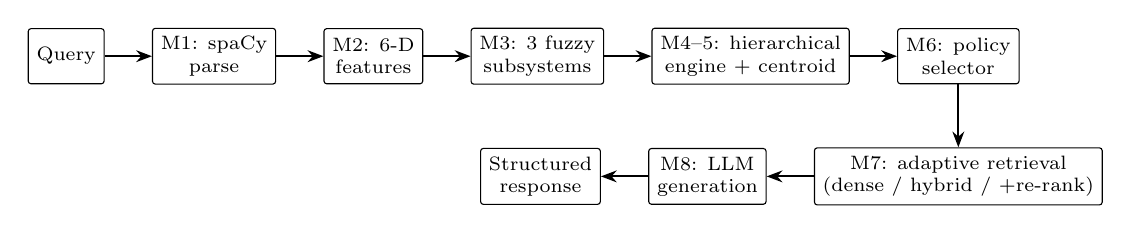
\begin{tikzpicture}[
  node distance=3mm and 6mm,
  box/.style={draw, rounded corners=1pt, align=center, font=\scriptsize, inner sep=3pt, minimum height=7mm},
  arr/.style={-{Stealth[length=2mm]}, thick}
]
\node[box] (q) {Query};
\node[box, right=of q] (pre) {M1: spaCy\\parse};
\node[box, right=of pre] (feat) {M2: 6-D\\features};
\node[box, right=of feat] (fuzzy) {M3: 3 fuzzy\\subsystems};
\node[box, right=of fuzzy] (hier) {M4--5: hierarchical\\engine + centroid};
\node[box, right=of hier] (pol) {M6: policy\\selector};
\node[box, below=8mm of pol] (retr) {M7: adaptive retrieval\\(dense / hybrid / +re-rank)};
\node[box, left=of retr] (llm) {M8: LLM\\generation};
\node[box, left=of llm] (ans) {Structured\\response};
\draw[arr] (q) -- (pre);
\draw[arr] (pre) -- (feat);
\draw[arr] (feat) -- (fuzzy);
\draw[arr] (fuzzy) -- (hier);
\draw[arr] (hier) -- (pol);
\draw[arr] (pol) -- (retr);
\draw[arr] (retr) -- (llm);
\draw[arr] (llm) -- (ans);
\end{tikzpicture}
\caption{Pipeline overview. Complexity is estimated \emph{before} retrieval
from the query alone; the selected policy then dictates which retrieval
components execute.}
\label{fig:pipeline}
\end{figure}

\subsection{Query preprocessing and feature extraction}
\label{sec:features}

Each query is parsed with spaCy's \texttt{en\_core\_web\_sm} pipeline
\citep{honnibal2020spacy} (tokenization, lemmatization, POS tagging, named
entity recognition, dependency parsing). From the parse we extract exactly six
scalar features (Table~\ref{tab:features}), each normalized to $[0,1]$ by a
documented cap $c$ via $\tilde{x} = \min(x/c, 1)$. No document retrieval
occurs at this stage; the features cost $\sim$75\,ms on CPU, dominated by the
spaCy parse.

\begin{table}[t]
\centering\small
\begin{tabular}{lllc}
\toprule
Category & Feature & Raw definition & Cap $c$ \\
\midrule
Linguistic & Query length & non-punctuation token count & 30 \\
Linguistic & Dependency depth & max depth of dependency tree & 10 \\
Knowledge & Entity density & named entities / tokens & 0.5 \\
Knowledge & Domain term density & weighted domain mass / tokens & 0.2 \\
Reasoning & Intent type & soft mixture over \{definition, procedure, reasoning, comparison\} & --- \\
Reasoning & Semantic ambiguity & mean WordNet polysemy of content words & 10 \\
\bottomrule
\end{tabular}
\caption{The six pre-retrieval features. Domain-term density and intent are
computed as described in \S\ref{sec:domain} and \S\ref{sec:intent};
ambiguity uses WordNet \citep{miller1995wordnet} synset counts.}
\label{tab:features}
\end{table}

\subsection{Corpus-derived domain vocabulary}
\label{sec:domain}

The domain-term density feature measures how much specialized terminology a
query contains. Rather than a hand-maintained keyword list (which must be
re-curated per deployment and cannot cover unseen corpora), we \emph{derive} a
weighted vocabulary from the ingested corpus, once, at index time, with no
training or labels:
(i) lemmatize every passage (keeping content nouns, adjectives, and verbs;
proper nouns are excluded as they are already captured by entity density);
(ii) score each term by its summed TF-IDF mass across passages
\citep{robertson2009bm25}, giving corpus salience;
(iii) \emph{contrastively} re-weight each term by a specificity factor
$\max(0, (Z_{\max}-z)/Z_{\max})$ where $z$ is the term's Zipf frequency in
general English, so corpus-frequent but generic words ("day", "company")
are suppressed and genuinely specialized terms ("encryption", "uptime",
"biometric") are promoted; (iv) keep the top-$N$ terms with weights rescaled to
$(0,1]$. Domain-term density is then the token-averaged sum of matched terms'
weights, so rare technical terms move the feature more than common ones. The
vocabulary is interpretable (a printable ranked list), corpus-adaptive (a new
corpus yields a new vocabulary automatically), and still training-free; a
hand-authored list can additionally be merged in as a supplement.

\subsection{Syntax-aware soft intent}
\label{sec:intent}

Intent is detected from lexical cues \emph{and} the dependency parse, and
returned as a continuous score rather than a hard class. Lexical regex families
provide first-pass evidence for each of \{definition, procedure, reasoning,
comparison\}. The parse then supplies structural evidence that surface patterns
miss: comparative morphology (\texttt{JJR}/\texttt{RBR} tags, e.g. ``faster'')
and coordinated nominal alternatives (``Postgres \emph{or} MySQL'') signal a
comparison even with no comparison keyword, while an ambiguous ``between $X$ and
$Y$'' is counted as a comparison only when $X,Y$ are nominal (so ``between 1990
and 1995'' is not). The final intent score is the evidence-weighted mixture of
the per-intent scalars (definition${=}0.10$, procedure${=}0.40$,
reasoning${=}0.70$, comparison${=}0.95$), with definition/procedure treated as
background question-framing that does not dilute a fired comparison/reasoning
intent. A single-intent query reproduces the hard scalar exactly; a genuinely
mixed query (``compare $X$ and $Y$ and explain why'') lands between anchors. The
classifier remains fully rule-based and training-free.

\subsection{Stage 1: three fuzzy expert subsystems}
\label{sec:subsystems}

All fuzzy variables share the universe $[0,1]$ and three overlapping
membership functions: $\mathrm{Low} = \mathrm{trap}(0,0,0.2,0.4)$,
$\mathrm{Medium} = \mathrm{tri}(0.25,0.5,0.75)$,
$\mathrm{High} = \mathrm{trap}(0.6,0.8,1,1)$. The overlapping supports
guarantee nonzero membership for every crisp input.

Instead of one flat rule base over six inputs, three two-input Mamdani
subsystems \citep{mamdani1975experiment} each produce one intermediate
complexity:
\begin{align*}
C_{\mathrm{ling}} &= F_L(\text{query length},\ \text{dependency depth}),\\
C_{\mathrm{know}} &= F_K(\text{entity density},\ \text{domain density}),\\
C_{\mathrm{reas}} &= F_R(\text{intent},\ \text{ambiguity}),
\end{align*}
each with a complete $3\times3 = 9$-rule base. The default output level is the
rounded mean of the two input levels; $F_R$ overrides the row where intent is
High so that a comparison intent alone forces high reasoning complexity
(\emph{if intent is comparison then reasoning complexity is high}),
implemented with scikit-fuzzy \citep{warner2019skfuzzy}.

\subsection{Stage 2: hierarchical aggregation and defuzzification}
\label{sec:hierarchical}

The second stage maps $(C_{\mathrm{ling}}, C_{\mathrm{know}},
C_{\mathrm{reas}})$ to an overall complexity. Because it operates on three
summarized inputs rather than six raw features, a compact rule base suffices.
We enumerate all $3^3 = 27$ level combinations and assign each an output level
by the \emph{level-sum} rule: with $\mathrm{Low}{=}0$, $\mathrm{Medium}{=}1$,
$\mathrm{High}{=}2$ and $s$ the sum over the three inputs,
\begin{equation}
\mathrm{Overall}(s) =
\begin{cases}
\mathrm{Low} & s \le 1,\\
\mathrm{Medium} & 2 \le s \le 3,\\
\mathrm{High} & s \ge 4.
\end{cases}
\label{eq:levelsum}
\end{equation}
The 27 combinations are compressed into three disjunctive Mamdani rules (one
per output level). Two properties follow directly from
Eq.~\eqref{eq:levelsum} and the overlapping memberships, and are locked in by
property-based tests:

\begin{itemize}
  \item \textbf{Completeness.} Every input triple activates at least one rule;
        no input produces an empty (undefined) output.
  \item \textbf{Monotonicity.} Raising any single input's level never lowers
        the output level; empirically, raising any crisp subsystem score never
        lowers the defuzzified overall score.
\end{itemize}

The aggregated output fuzzy set is defuzzified by the centroid method into a
continuous complexity score $s^\ast \in [0,1]$. The example rules from the
design specification are special cases of Eq.~\eqref{eq:levelsum}: all-Low
$\Rightarrow$ Low ($s{=}0$); Linguistic High $\wedge$ Knowledge High
$\Rightarrow$ High ($s \ge 4$); Medium--Medium--Low $\Rightarrow$ Medium
($s{=}2$).

\subsection{Retrieval policy selection}
\label{sec:policy}

The score maps to a policy through configurable bands
(Table~\ref{tab:policy}). Thresholds, top-$k$ values, and re-ranking flags are
configuration, not code.

\begin{table}[t]
\centering\small
\begin{tabular}{lccl}
\toprule
Score band & Class & Top-$k$ & Strategy \\
\midrule
$[0.00, 0.35)$ & Simple & 2 & dense retrieval only \\
$[0.35, 0.70)$ & Medium & 5 & hybrid BM25 + dense (RRF) \\
$[0.70, 1.00]$ & Complex & 10 & hybrid + cross-encoder re-ranking \\
\bottomrule
\end{tabular}
\caption{Retrieval policy bands (defaults; all values configurable).}
\label{tab:policy}
\end{table}

\subsection{Adaptive retrieval and generation}
\label{sec:retrieval}

\textbf{Dense retrieval} encodes queries and passages with a MiniLM bi-encoder
\citep{reimers2019sbert} (all-MiniLM-L6-v2); L2-normalized embeddings reduce
cosine similarity to a dot product over a precomputed index.
\textbf{Sparse retrieval} uses BM25 \citep{robertson2009bm25}.
\textbf{Hybrid fusion} combines the two ranked lists with reciprocal rank
fusion \citep{cormack2009rrf}:
\begin{equation}
\mathrm{RRF}(d) = \sum_{r \in \mathcal{R}} \frac{1}{k + \mathrm{rank}_r(d)},
\qquad k = 60,
\end{equation}
chosen over score interpolation because BM25 and cosine scores are on
incomparable scales and rank fusion requires no per-query normalization or
weight tuning. \textbf{Re-ranking} (Complex tier only) scores
(query, passage) pairs with a MiniLM cross-encoder
\citep{nogueira2019rerank} over a 50-candidate fused pool and keeps the top
10.

\textbf{Generation} uses a \emph{retrieve-then-focus} scheme: the policy's
full top-$k$ is retrieved (recall), but only the $n{=}3$ best-ranked passages
enter the prompt of the answering model, Flan-T5-base \citep{chung2024flan}
(250M parameters, CPU). Small readers degrade sharply when fed many passages;
in preliminary experiments, prompting with all 10 passages collapsed
enterprise-benchmark F1 from $0.92$ to $0.03$. The reader is a swappable
interface; nothing in the routing depends on it.

\section{Experimental Setup}
\label{sec:setup}

\paragraph{Corpora and question sets.}
(i) \textbf{SQuAD-200}: 300 unique passages from the SQuAD~v1.1 validation
split \citep{rajpurkar2016squad} and 200 questions constrained to one question
per passage, so gold passages span 200 distinct documents (unconstrained
sampling collapses onto a handful of contexts because SQuAD groups many
questions per context). (ii) \textbf{Enterprise-22}: an internal-knowledge-base
benchmark of 20 authored corporate policy documents (56 chunked passages) with
22 hand-labeled (question, answer, gold passage) triples spanning HR, security,
privacy/GDPR, product, and engineering topics; it represents the
enterprise-assistant workload that motivates this work.

\paragraph{Baselines.}
Traditional fixed-strategy RAG at both extremes, holding every component
except routing identical: \textbf{fixed-simple} (always top-2 dense) and
\textbf{fixed-complex} (always top-10 hybrid + cross-encoder). The adaptive
system and both baselines share the same indexes, models, prompt, and reader.

\paragraph{Metrics.}
Retrieval: recall@$k$ (does the gold passage appear in the retrieved set,
$k$ per strategy). Answer quality: SQuAD-normalized token-level F1 and exact
match against gold answers. Cost: mean end-to-end latency per query
(single-threaded CPU), mean documents retrieved, and the fraction of queries
on which the cross-encoder ran. One untimed warm-up query exercising every
lazily-loaded component (query encoder, cross-encoder, reader) precedes
timing, so one-time model loading is excluded from per-query latency; without
it, whichever strategy first triggers a lazy load absorbs the load time into
its mean, which materially skews small-$n$ comparisons.

\paragraph{Implementation.}
Python 3.11 on Windows 11, CPU only (Intel Core i7-13650HX, 16\,GB RAM; no
GPU used).
spaCy \texttt{en\_core\_web\_sm}; scikit-fuzzy 0.5 (Mamdani, centroid);
sentence-transformers all-MiniLM-L6-v2 and
cross-encoder/ms-marco-MiniLM-L-6-v2; rank\_bm25; google/flan-t5-base. The
pipeline is deterministic (greedy decoding, fixed rules), so results are
reproducible modulo latency noise. All code, corpora, gold labels, configs,
and a 36-test suite (feature extraction, fuzzy boundary and monotonicity
properties, policy thresholds, end-to-end smoke test) accompany this paper.

\section{Results}
\label{sec:results}

\subsection{Open-domain benchmark (SQuAD-200)}

\begin{table}[t]
\centering\small
\begin{tabular}{lcccccc}
\toprule
Strategy & Recall@$k$ & F1 & EM & Latency (s) & Docs/query & Re-rank \% \\
\midrule
fixed-simple  & \sqSiRec & \sqSiFone & \sqSiEM & \sqSiLat & \sqSiDocs & \sqSiRr \\
fixed-complex & \sqCoRec & \sqCoFone & \sqCoEM & \sqCoLat & \sqCoDocs & \sqCoRr \\
\textbf{adaptive} & \textbf{\sqAdRec} & \sqAdFone & \sqAdEM & \sqAdLat & \sqAdDocs & \sqAdRr \\
\bottomrule
\end{tabular}
\caption{SQuAD-200 results (200 questions, 300-passage corpus, CPU). Adaptive
routing recovers $73\%$ of the recall gap between the fixed baselines while
re-ranking only \sqAdRr\% of queries at roughly one third of fixed-complex's
latency. Class distribution chosen by the router: Simple \sqSimple, Medium
\sqMedium, Complex \sqComplex. Reader-side F1/EM \emph{anti}-correlate with
context size (see text).}
\label{tab:squad}
\end{table}

Table~\ref{tab:squad} shows the main result. On the retrieval side, the
pattern is exactly as motivated: the cheap baseline's shallow top-2 retrieval
misses the gold passage on a quarter of the questions (recall \sqSiRec); the
expensive baseline reaches recall \sqCoRec\ but pays $10$ documents plus a
cross-encoder pass on every query; the adaptive router attains recall
\sqAdRec---closing $75\%$ of the gap, within $6$ points of the
ceiling---while retrieving \sqAdDocs\ documents per query on average,
re-ranking \sqAdRr\% of queries, and running at close to one third of
fixed-complex's latency (\sqAdLat\,s vs.\ \sqCoLat\,s).

The reader-side metrics tell a different---and instructive---story: F1
\emph{decreases} monotonically with retrieval depth (\sqSiFone\ for top-2
dense, \sqAdFone\ for adaptive, \sqCoFone\ for top-10 hybrid+re-rank), the
opposite ordering of recall. Two mechanisms explain the inversion. First,
\emph{context sensitivity}: a 250M-parameter extractive reader is easily
distracted; each additional or lexically-fused passage in the prompt raises
the chance it extracts a plausible span from the wrong passage, and this loss
outweighs the recall gain at this reader scale. Second, a dataset confound:
SQuAD-format QA is part of Flan-T5's instruction-tuning mixture
\citep{chung2024flan}, so the reader can sometimes answer from parametric
memory even when retrieval fails, further muting the dependence of F1 on
recall. We therefore treat retrieval effectiveness per unit cost as the
primary endpoint on this benchmark and F1/EM as a secondary, reader-bound
signal; \S\ref{sec:limits} discusses when recall gains should convert into
answer-quality gains (stronger readers, corpora outside the reader's training
distribution---as in the enterprise benchmark below, where no leakage is
possible and quality ties at ceiling instead of inverting).

\subsection{Enterprise benchmark (Enterprise-22)}

\begin{table}[t]
\centering\small
\begin{tabular}{lcccccc}
\toprule
Strategy & Recall@$k$ & F1 & EM & Latency (s) & Docs/query & Re-rank \% \\
\midrule
fixed-simple  & \enSiRec & \enSiFone & \enSiEM & \enSiLat & \enSiDocs & \enSiRr \\
fixed-complex & \enCoRec & \enCoFone & \enCoEM & \enCoLat & \enCoDocs & \enCoRr \\
\textbf{adaptive} & \enAdRec & \enAdFone & \enAdEM & \textbf{\enAdLat} & \textbf{\enAdDocs} & \textbf{\enAdRr} \\
\bottomrule
\end{tabular}
\caption{Enterprise-22 results (warmed-up timing). On a small, clean corpus
every strategy retrieves the gold passage, so quality ties and the comparison
isolates cost: adaptive matches fixed-complex quality at $1.6\times$ lower
latency and $9.1$\% re-ranker usage. Router distribution: Simple 4 (18.2\%),
Medium 16 (72.7\%), Complex 2 (9.1\%).}
\label{tab:enterprise}
\end{table}

On the enterprise corpus (Table~\ref{tab:enterprise}) all strategies achieve
perfect recall---with 56 clean passages even top-2 dense retrieval
suffices---so the benchmark isolates the cost dimension. Adaptive matches
fixed-complex on every quality metric while cutting mean latency from
\enCoLat\,s to \enAdLat\,s ($1.6\times$), documents per query from \enCoDocs\
to \enAdDocs, and cross-encoder usage from 100\% to \enAdRr\%. Unlike
SQuAD-200, quality here does \emph{not} invert with depth: with clean,
topically-distinct passages and a leakage-free corpus, the focused prompt
contains the same gold passage under every strategy, and all three tie at the
reader's ceiling.

\subsection{Routing behavior and interpretability}

The router's decisions are inspectable end to end. Two contrasting Complex
routings illustrate that the subsystems capture distinct phenomena:

\begin{itemize}
\item \emph{``Compare the data-retention obligations under GDPR and CCPA for
cloud providers processing biometric data''} $\rightarrow$ score $0.844$
(Complex) driven by \textbf{Knowledge} (domain density $1.0$) and
\textbf{Reasoning} (comparison intent $0.95 \Rightarrow C_{\mathrm{reas}} =
0.83$), with Linguistic moderate ($0.50$).
\item \emph{``What are the differences between the Starter, Growth, and
Enterprise subscription tiers?''} $\rightarrow$ score $0.844$ (Complex) driven
instead by \textbf{Linguistic} (dependency depth $0.8 \Rightarrow
C_{\mathrm{ling}} = 0.83$) and \textbf{Reasoning} ($0.84$), with Knowledge low
($0.16$; no domain keywords).
\end{itemize}

Conversely, \emph{``What is GDPR?''} scores $0.156$ (Simple): despite a domain
keyword, its brevity, definition intent, and shallow parse keep every
subsystem low. The specification's calibration pair---this query Low, the
GDPR/CCPA comparison High---is satisfied with a wide margin
($0.156$ vs.\ $0.844$ against thresholds $0.35$/$0.70$).

\subsection{Cost analysis}

Let $c_{\mathrm{rr}}$ denote the cross-encoder cost per query. Fixed-complex
pays $c_{\mathrm{rr}}$ always; adaptive pays it on the Complex fraction only
($5$--$9\%$ across our benchmarks, an $11$--$20\times$ reduction), plus a
routing overhead of $\sim$75\,ms (spaCy parse + fuzzy inference; the
corpus vocabulary is loaded once at startup, not per query), which is one to two
orders of magnitude cheaper than the re-ranking it avoids and is independent of
corpus size. Retrieval volume follows the workload mix: the per-class top-$k$
values weighted by the router's class distribution, empirically about half of
fixed-complex volume on both benchmarks (\sqAdDocs\ and \enAdDocs\ vs.\ $10$
documents per query).

\section{Limitations}
\label{sec:limits}

\textbf{Reader ceiling and context sensitivity.} With a 250M-parameter
reader, end-to-end F1/EM are reader-bound, and on SQuAD-200 they
\emph{anti}-correlate with retrieval depth: the reader is distracted by
additional context faster than it benefits from higher recall
(\S\ref{sec:results}). Retrieval-side gains should convert into answer
quality only with a stronger reader (the LLM interface is swappable, e.g., to
a local Llama via Ollama); verifying that conversion is future work.
\textbf{Training-data leakage.} SQuAD-format QA appears in Flan-T5's
instruction-tuning mixture \citep{chung2024flan}, so on SQuAD-200 the reader
can sometimes answer from parametric memory, inflating all strategies' F1/EM
and further decoupling them from retrieval quality; the enterprise benchmark,
authored for this work, is leakage-free by construction. \textbf{Rule
priors.} Two of the strongest priors are removed: the domain vocabulary is
derived from the corpus rather than hand-listed (\S\ref{sec:domain}), and intent
uses the dependency parse rather than keywords alone (\S\ref{sec:intent}) --
both still training-free. What remains hand-specified is the numeric scaffolding
(normalization caps, membership breakpoints, intent scalars, policy thresholds),
which encodes designer judgment and may be miscalibrated for query distributions
unlike those studied here (e.g., non-English or conversational queries);
learning it from logged traces while keeping the rules interpretable is future
work. \textbf{Benchmark scale.} Our
benchmarks (200 and 22 questions, single machine, single run) support the
cost/recall conclusions but are too small for fine-grained quality
distinctions; latencies are indicative, not rigorous. \textbf{No
multi-step retrieval.} We route among single-shot retrieval policies;
integrating iterative strategies \citep{jiang2023flare,jeong2024adaptive} as a
fourth tier is natural future work, as is learning the membership breakpoints
from logged traces while retaining the interpretable rule structure.

\section{Conclusion}

We presented a retrieval-augmented generation architecture that replaces the
conventional fixed retrieval configuration with per-query routing by a
hierarchical fuzzy inference engine over six pre-retrieval features. The
router is training-free, interpretable, and adds negligible overhead, and its
rule base is complete and monotonic by construction. Across an open-domain and
an enterprise benchmark, adaptive routing consistently delivered close to the
expensive baseline's retrieval effectiveness at a small fraction of its
cost---cutting latency by $1.6$--$2.8\times$, retrieval volume by roughly
half, and cross-encoder invocations by an order of magnitude---while remaining
fully explainable. We release the complete
system, corpora, and harness to support reproduction and extension.

\paragraph{Reproducibility.}
All numbers in Tables~\ref{tab:squad} and \ref{tab:enterprise} regenerate from
the released repository with two commands (\texttt{rag ingest},
\texttt{rag eval}) per benchmark; routing traces print with
\texttt{rag ask -v}; the property tests run with \texttt{pytest}.

\bibliographystyle{plainnat}
\bibliography{references}

\end{document}
